\documentclass[12pt,]{article}
\usepackage{lmodern}
\usepackage{amssymb,amsmath}
\usepackage{ifxetex,ifluatex}
\usepackage{fixltx2e} % provides \textsubscript
\ifnum 0\ifxetex 1\fi\ifluatex 1\fi=0 % if pdftex
  \usepackage[T1]{fontenc}
  \usepackage[utf8]{inputenc}
\else % if luatex or xelatex
  \ifxetex
    \usepackage{mathspec}
  \else
    \usepackage{fontspec}
  \fi
  \defaultfontfeatures{Ligatures=TeX,Scale=MatchLowercase}
\fi
% use upquote if available, for straight quotes in verbatim environments
\IfFileExists{upquote.sty}{\usepackage{upquote}}{}
% use microtype if available
\IfFileExists{microtype.sty}{%
\usepackage{microtype}
\UseMicrotypeSet[protrusion]{basicmath} % disable protrusion for tt fonts
}{}
\usepackage[margin=1in]{geometry}
\usepackage{hyperref}
\hypersetup{unicode=true,
            pdftitle={DFO Multispecies Survey Trip Report},
            pdfauthor={Science Branch},
            pdfborder={0 0 0},
            breaklinks=true}
\urlstyle{same}  % don't use monospace font for urls
\usepackage{graphicx,grffile}
\makeatletter
\def\maxwidth{\ifdim\Gin@nat@width>\linewidth\linewidth\else\Gin@nat@width\fi}
\def\maxheight{\ifdim\Gin@nat@height>\textheight\textheight\else\Gin@nat@height\fi}
\makeatother
% Scale images if necessary, so that they will not overflow the page
% margins by default, and it is still possible to overwrite the defaults
% using explicit options in \includegraphics[width, height, ...]{}
\setkeys{Gin}{width=\maxwidth,height=\maxheight,keepaspectratio}
\IfFileExists{parskip.sty}{%
\usepackage{parskip}
}{% else
\setlength{\parindent}{0pt}
\setlength{\parskip}{6pt plus 2pt minus 1pt}
}
\setlength{\emergencystretch}{3em}  % prevent overfull lines
\providecommand{\tightlist}{%
  \setlength{\itemsep}{0pt}\setlength{\parskip}{0pt}}
\setcounter{secnumdepth}{0}
% Redefines (sub)paragraphs to behave more like sections
\ifx\paragraph\undefined\else
\let\oldparagraph\paragraph
\renewcommand{\paragraph}[1]{\oldparagraph{#1}\mbox{}}
\fi
\ifx\subparagraph\undefined\else
\let\oldsubparagraph\subparagraph
\renewcommand{\subparagraph}[1]{\oldsubparagraph{#1}\mbox{}}
\fi

%%% Use protect on footnotes to avoid problems with footnotes in titles
\let\rmarkdownfootnote\footnote%
\def\footnote{\protect\rmarkdownfootnote}

%%% Change title format to be more compact
\usepackage{titling}

% Create subtitle command for use in maketitle
\newcommand{\subtitle}[1]{
  \posttitle{
    \begin{center}\large#1\end{center}
    }
}

\setlength{\droptitle}{-2em}

  \title{DFO Multispecies Survey Trip Report}
    \pretitle{\vspace{\droptitle}\centering\huge}
  \posttitle{\par}
  \subtitle{Newfoundland and Labrador Region}
  \author{Science Branch}
    \preauthor{\centering\large\emph}
  \postauthor{\par}
    \date{}
    \predate{}\postdate{}
  

\begin{document}
\maketitle

\subsection{TRIP SUMMARY}\label{trip-summary}

\textbf{Vessel:} Teleost \textbar{} \textbf{Trip number:} TEL190

\textbf{Sailed from:} St.~Anthony, NL \textbar{} \textbf{Returned to:}
St.~John's, NL

\textbf{Start Date:} October 24, 2018 \textbf{End Date:} November 6,
2018

\textbf{Scientific Staff:} Laura Wheeland(SIC), F. Dawson, K. Rideout,
M. Terry, B. Vaters, P. Higdon, J. Croft, F. Tulk, T. Bungay

This report has been prepared by Laura Wheeland(SIC).

\textbf{Area of Operation:} NAFO Divisions 2H and 2J fishing in depths
to a maximum of 1334 meters.

\textbf{Purpose:}

\textbf{Fishing Methods:}

\subsection{Catch Summary}\label{catch-summary}

This trip completed 35 sets in NAFO divisions 2J, 2H. Total catch was
6961kg, with 167 taxa recorded. Fishing occurred from 129m to 1334m.\\

\begin{center}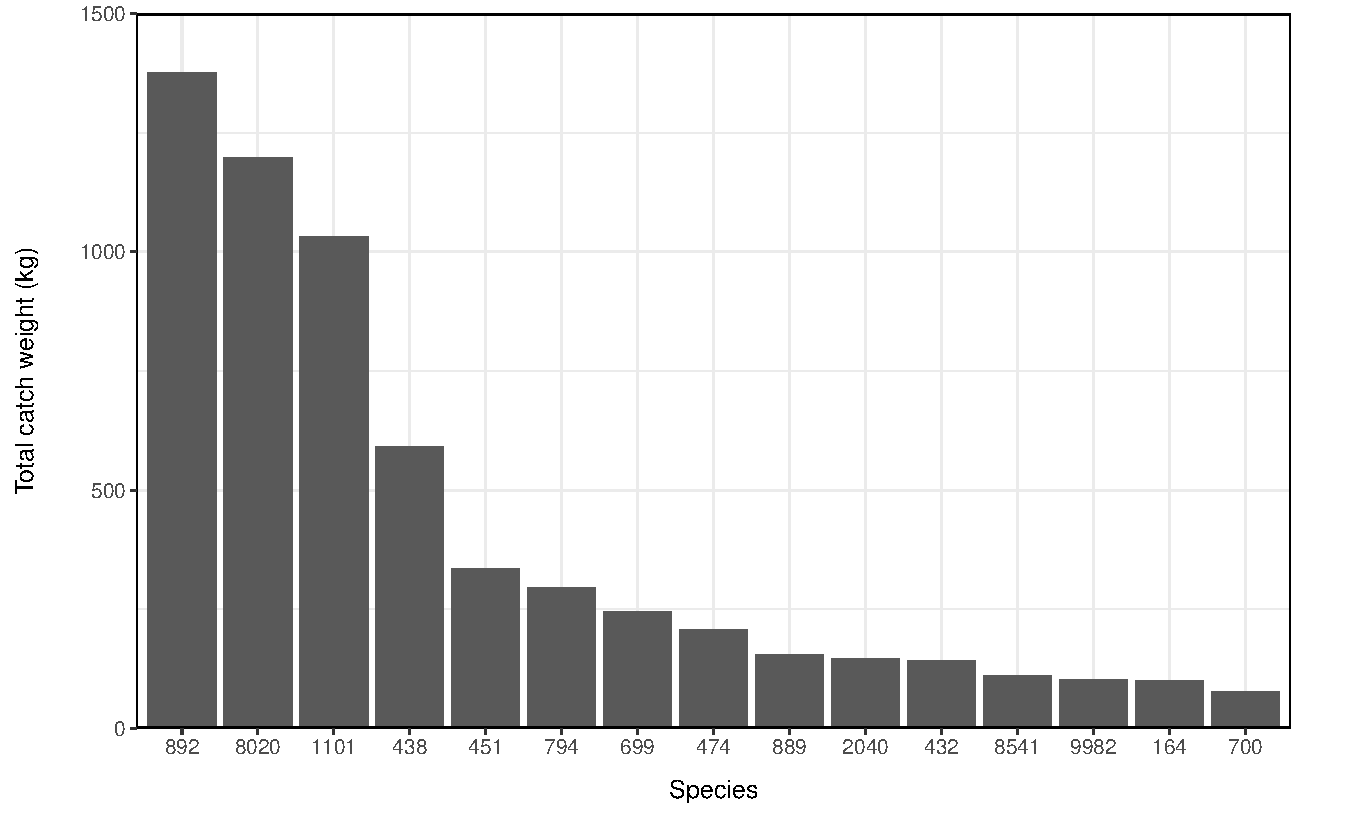
\includegraphics[width=6in]{knitr-figs/catch.plot-1} \end{center}

\emph{Figure 1: Total catch weight of the fifteen most commonly
encountered taxa during trip TEL190}

\section{}\label{section}

\section{\texorpdfstring{\texttt{\{r\ Sets.Table,\ echo=FALSE\}\ \#\ \#n\_sets\ \textless{}-\ RV.SET\ \%\textgreater{}\%\ \ \#\ \ group\_by(depth.bin)\ \%\textgreater{}\%\ \ \#\ \ summarize(N=n())\ \ \#\ \#\ \#}}{\{r Sets.Table, echo=FALSE\} \# \#n\_sets \textless{}- RV.SET \%\textgreater{}\%  \#  group\_by(depth.bin) \%\textgreater{}\%  \#  summarize(N=n())  \# \# \#}}\label{r-sets.table-echofalse-n_sets---rv.set-group_bydepth.bin-summarizenn}

\section{\texorpdfstring{kable(n\_sets,
format=``markdown'')}{kable(n\_sets, format=markdown)}}\label{kablen_sets-formatmarkdown}


\end{document}
